\chapter{Hilfsgelder}
\label{chap:Hilfsgelder}
Zum Abschluss der Beispiele soll eine Anwendung von Smart Contracts aufgezeigt werden, die sich grundlegend von den anderen bereits vorgestellten unterscheidet. Wurde bisher immer von einem Business-Use-Case ausgegangen, können auch komplett unterschiedliche Felder von Smart Contracts profitieren. So auch die Verteilung von Hilfsgeldern, wie sie unter anderem von der UN gepflegt wird. 

Eines der Felder der Vereinten Nationen ist die weltweite Hungerbekämpfung mithilfe des \emph{World Food Programme (WFP)}. Die Zahlen zeugen von dem enormen Ausmaß der Hilfeleistungen: So wurden im Jahr 2018 über das WFP mehr als 1,6 Milliarden US-Dollar an Hilfsgeldern in Form von Bargeld an Bedürftige vergeben. Zuvor wurden in größeren Mengen Sachgüter vergeben, was jedoch auf der einen Seite keinen Beitrag zur dortigen Wirtschaft leistet, als auch die Flexibilität der Hilfeempfänger einschränkt. Im Umkehrschluss muss dabei seitens der Organisation auch dem Missbrauch der Gelder vorgebeugt werden. So besteht die Gefahr, dass über Mehrfachidentitäten unberechtigt Geld erschlichen werden kann. Auch auf Seiten der Banken ist man in instabilen Regionen dieser Erde nicht vor Unterschlagungen geschützt. Um diese Faktoren ausschließen zu können, wird seit 2017 in dem Projekt \emph{Building Blocks} jede Auszahlung über die Ethereum Blockchain authentifiziert und registriert. Sollten die erhaltenen und die zustehenden Leistungen divergieren, können daher Unregelmäßigkeiten aufgedeckt und dem Missbrauch von Spenden entgegengewirkt werden. Darüber hinaus ergeben sich nach eigenen Angaben der UN Kosteneinsparungen in Höhe von bis zu 98 \%. Das resultiert unter anderem aus dem Wegfall der an den Transaktionen beteiligten Intermediären, wie beispielsweise Banken. Dadurch kommt auch ein höherer Prozentsatz der Gelder direkt bei den Betroffenen an. Eine Verfeinerung der Technologie ergibt sich mit der Hinzunahme von Iris-Daten, wie sie als eindeutige Identifizierungsmöglichkeit an immer mehr Stellen eingesetzt wird (siehe Abbildung \ref{fig:IrisSystem}). Davor konnten Hilfsbedürftige mittels an Geldautomaten installierten Iris-Scannern, ohne PIN-Code oder sonstige Identifikation, Bargeld abheben. Jetzt können Lebensmitteleinkäufe komplett bargeldlos und sicher auf der Blockchain abgewickelt werden. Nach ersten Tests in Pakistan wurde das System auf Flüchtlingsunterkünfte in Jordanien ausgeweitet. Hier weichen die Zahlen ab; in einer Quelle ist von 10 000 Personen die Rede, in der anderen um einen Faktor zehn multiplizierten Wert. Nichtsdestotrotz zeigt dieses Beispiel, dass es sich hierbei um größere Maßstäbe handelt. \cite[vgl.][]{WFP2019, WFPBlockchain2018}

\begin{figure}[h!]
  \centering
  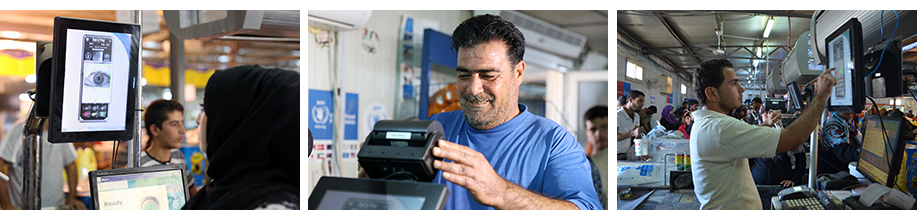
\includegraphics[width=\textwidth]{Bilder/Iris-Scan.jpg}
  \caption[Iris-System der UN]{Iris-System der UN \cite{WTWebsite2019}}
  \label{fig:IrisSystem}
\end{figure}

Wie das System im Hintergrund genau funktioniert und mit der im Detail Blockchain interagiert, ist unklar. Dies dürfte aber auch der Identitätssicherung der Flüchtlinge und Hilfeempfänger geschuldet sein. Dabei gilt es anzumerken, dass das Iris-System offline arbeitet und die Einträge in der Blockchain vermutlich nur über Identifikationsnummern realen Personen zugeordnet werden können. Wie viele Smart Contracts eingesetzt werden, lässt sich auch nur spekulieren. Bei der Abprüfung von zustehenden Leistungen ist aber die Nutzung eines Contracts wahrscheinlich, ähnelt sie doch beispielsweise der Kontostandsabfrage aus dem Dachser-Beispiel.\\
Wieviel an den Transaktionskosten in absoluten Zahlenwerten gespart wird, wird von der UN nicht genannt. Dies wäre eine interessante Kennzahl gewesen, betrachtet man die stark schwankenden Transaktionskosten für das Mining bei Kryptowährungen und dem Bestätigen von Transaktionen. \\
In Anbetracht der desolaten Lage in den Flüchtlingsgebieten wird der Sicherheitsaspekt durch die Nachvollziehbarkeit aller einzelnen Transaktionen und deren Zuordnung zu Personen verständlich. Dass so etwas aber in Ländern wie Deutschland Datenschutzbedenken hervorrufen würde, gilt als wahrscheinlich.

%Mehr Sicherheit für UN wegen Missbrauch - Datenschutzbedenken wären vor allem in Deutschland, Iris-System nicht an das Internet angeschlossen

